%!TEX root = ../memoire.tex

\chapter{Adaptation de GenDR}\label{ch:implementation}

Au chapitre précédent, nous avons expliqué comment nous avons extrait les informations de VerbNet à l'aide de scripts Python pour les importer dans GenDR. Ce chapitre couvrira l'adaptation de ce réalisateur pour lui faire exploiter ces nouvelles données. D'abord, nous expliquerons comment nos dictionnaires fonctionnent après l'importation de VerbNet et comment ils communiquent entre eux. Puis, nous montrerons comment fonctionnent les nouvelles règles de grammaire qui activent ces connaissances lexicales.

\section{Adaptation des dictionnaires}

Au chapitre \ref{chapgendr}, nous avons montré comment le lexique s'encodait dans GenDR. Nous avions deux dictionnaires: un dictionnaire de sémantèmes (\emph{semanticon}) et un dictionnaire de lexèmes (\emph{lexicon}). À la suite des informations extraites sur les \acp{GP}, nous avons maintenant un dictionnaire de \acp{GP} (\emph{gpcon}), ce qui implique un changement important de l'architecture du \emph{lexicon} et des règles de la grammaire (surtout pour les règles de correspondance sémantique).

\subsection{Une nouvelle architecture pour le \emph{lexicon}}

Le \emph{lexicon} de GenDR est maintenant séparé en quatre sections: les classes abstraites, les verbes de VerbNet, les classes verbales de VerbNet et le reste du lexique.

La première section, \textbf{\texttt{ABSTRACT CLASSES}}, décrit les classes générales de GenDR. Elle donne les propriétés génériques des verbes, noms, adverbes, adjectifs, prépositions, etc.

Dans la version originale de GenDR, les comportement syntaxiques \textbf{des verbes} étaient décrits dans cette section. Il y avait une hiérarchie rudimentaire de classes de verbes (intransitif, transitif direct/indirect et ditransitif) comprenant toute l'information syntaxique (les patrons de régime) pour chaque sous-classe. Maintenant, la classe générale \texttt{VERB} ne contient que les informations partagées par tous les verbes du dictionnaire: soit, sa partie du discours profonde et celle de surface. 

Les autres catégories syntaxiques comme les noms ou les adjectifs contiennent plus d'information que la classe abstraite \texttt{VERB}. Puisque leurs comportements sont prévisibles, contrairement aux verbes. On encode: la partie du discours, un patron de régime par défaut et des traits morpho-syntaxiques lorsque c'est nécessaire. Par contre, comme on peut le voir dans la classe \texttt{NOUN}, on n'a pas l'information syntaxique explicite que donnent les patrons de régime, on n'a que l'identifiant de celui-ci, car les propriétés de chaque patron de régime, peu importe la catégorie syntaxique, sont encodées dans le dictionnaire prêt à cet effet (\emph{gpcon}).\FL{reformuler ce paragraphe}

\begin{lstlisting}[language=mate, caption = Extrait du \emph{lexicon}: attributs par défaut des classes génériques, label=classedef]
verb {
  dpos = V
  spos = verb
}

noun {
  dpos = N
  spos = noun
  countable = yes
  gp = { id=NP dia=1}
}
...
\end{lstlisting}

La deuxième section, \textbf{\texttt{VERBNET MEMBERS}}, contient les membres des classes verbales de VerbNet que nous avons extraits (voir figure~\ref{scriptmember}). Sont ici listés tous les 6\,393 verbes avec la classe de VerbNet (ou la sous-classe) à laquelle ils appartiennent.

\begin{lstlisting}[language=mate, caption = Extrait du \emph{lexicon}: unités lexicales verbales]
"open up" : "establish-55.5-1"
operate : "other_cos-45.4"
oppose : "amalgamate-22.2-3"
ordain : "appoint-29.1"
order_1 : "get-13.5.1"
order_2 : "order-60-1"
organize_1 : "create-26.4"
organize_2 : "establish-55.5-1"
organize_3 : "force-59-1"
originate : "establish-55.5-1"
ornament_1 : "butter-9.9"
ornament_2 : "fill-9.8"
ornament_3 : "illustrate-25.3"
...
\end{lstlisting}

La troisième section, \textbf{\texttt{VERBNET CLASSES}}, liste les types de \acp{GP} que sélectionne chaque classe verbale. Cela se modélise par un trait \texttt{gp} dont la valeur est une structure qui contient deux attributs: la diathèse (\texttt{dia}) et l'identifiant du patron de régime (\texttt{id}). La diathèse d'un \ac{GP} s'encode ainsi différement dans le nouveau \emph{lexicon}. 

Anciennement, la diathèse était explicitée dans l'entrée \texttt{predicate}, qui donnait une diathèse triviale par défaut à tous les prédicats du dictionnaire, mais qu'on pouvait court-circuiter pour un lexème donné. Maintenant, on spécifie pour chaque \ac{GP} la diathèse qui lui est associée de cette manière: \texttt{dia=132}\FL{faut utiliser une convention typographique pour les éléments de code, à revoir}, qui implique: \texttt{I:1 II:3 III:2}. Autrement dit, l'ordre de présentation des actants sémantiques (les chiffres arabes 1,3,2) correspondra à la réalisation syntaxique de ces actants (I,II,III). L'architecture de VerbNet ne nous permettait pas d'en extraire la diathèse, car cette ressource identifie les actants syntaxiques à l'aide des rôles thématiques. Ainsi, nous ne pouvions pas déduire la diathèse à partir des rôles, donc nous avons dû coder manuellement chaque diathèse de chaque \ac{GP}. Nous avons ajouté la valeur \texttt{dia} après l'importation de VerbNet dans GenDR. Puis, chaque classe verbale est dotée d'un trait \texttt{id}, l'identifiant du patron de régime, qui permettra au système de récupérer les propriétés syntaxiques du patron de régime correspondant.

Toutefois, nous avons relevé un problème important après avoir manuellement encodé chaque diathèse. En faisant quelques tests préliminaires pour tester notre système nous en sommes venus à la conclusion que le mécanisme d'héritage que nous postulions ne transmettait pas toutes les informations que nous souhaitions. Il se trouve que la partie du discours se transmet sans problème, mais les patrons de régime ne percolent pas entre les classes verbales. 

En effet, si un verbe pointe vers une sous-classe $X$, il héritera de ses patrons de régime, et il héritera de la partie du discours verbale qui est encodée dans la classe abstraite \texttt{VERB}, mais il n'héritera pas des patrons de régime encodés dans la classe mère de la sous-classe $X$. Le problème provient du fait que l'architecture que nous avons instaurée bloque l'héritage du trait \texttt{gp}, puisqu'on redéfinit complètement cet attribut dans la sous-classe. Ainsi, le système est incapable de récupérer les \acp{GP} encodés dans la classe dominante. Quant au trait \texttt{dpos}, il a pu se transmettre de sous-classes en classes jusqu'à la classe abstrait parce qu'il n'est jamais redéfini.\draft{il faudrait que tu me réexpliques brièvement pourquoi ça bloque, c'est parce qu'on le redéfini et qu'il perd ses propriétés précédentes ?}\FL{c'est un choix de design dans l'implémentation de MATE} Cela a eu pour conséquence que nous avons dû manuellement rajouter chaque \ac{GP} de classe dominantes à classes dominées, puisque les traits \texttt{dia} avaient déjà été manuellement encodés et qu'il aurait été plus coûteux de regénérer la structure automatiquement, perdant du coup ces diathèses.

\begin{lstlisting}[language=mate, caption = Extrait du \emph{lexicon}: classes de VerbNet, label=fig:vnclass]
"escape-51.1": verb {
  gp = { id=NP_V                           dia=1 } // The prisoners advanced.
  gp = { id=NP_V_PP_PATH_initial_loc       dia=1 } // He came from France.
  gp = { id=NP_V_PP_PATH_destination       dia=13 } // He came to Colorado.
  gp = { id=NP_V_PP_PATH_trajectory        dia=14 } // He came through the door.
  gp = { id=NP_V_PP_PATH_initial_loc_PP_PATH_destination dia=123 } // He came from France to Colorado.
  }
"escape-51.1-1": "escape-51.1" {
  gp = { id=NP_V                           dia=1 } // The prisoners advanced.
  gp = { id=NP_V_PP_PATH_initial_loc       dia=1 } // He came from France.
  gp = { id=NP_V_PP_PATH_destination       dia=13 } // He came to Colorado.
  gp = { id=NP_V_PP_PATH_trajectory        dia=14 } // He came through the door.
  gp = { id=NP_V_PP_PATH_initial_loc_PP_PATH_destination dia=123 } // He came from France to Colorado.
  gp = { id=NP_V_NP                        dia=12 } // The convict escaped the prison.
}
}...
\end{lstlisting}

Passons ensuite à la section \texttt{NON-VERBAL LEXICAL ENTRIES} qui regroupe \textbf{le reste du lexique}: noms, adjectifs, adverbes, prépositions, déterminants, etc. Ces entrées proviennent de la version originale de GenDR \citep{lareau18} et le contenu de cette section a été enrichi par les lexèmes qu'on retrouvait dans les phrases exemples de VerbNet. Bref, les entrées de cette section pointent vers les classes (\texttt{NOUNS}, \texttt{PREPOSITIONS}, \ldots) abstraites leur correspondant, ce qui leur permet d'hériter des attributs suivants: \texttt{dpos},\texttt{spos}, \texttt{id}, et \texttt{dia}.

\begin{lstlisting}[language=mate, caption = Extrait du \emph{lexicon}: unités lexicales non-verbales]
accountant : noun
acorn : noun
acquaitance  : noun
across : preposition
...
\end{lstlisting}

\subsection{Le dictionnaire des patrons de régime: \emph{gpcon}}

Le \emph{gpcon} est un dictionnaire de patrons de régime qui contient 278 identifiants uniques de \acp{GP} et leurs propriétés syntaxiques. Considérant que les classes verbales du lexicon partagent ces patrons de régime, l'option de les encoder dans un dictionnaire à part nous apparaît évidente. Cela allège grandement le contenu du lexicon et ça nous permet d'entretenir les données plus facilement. Ainsi, la modification d'un \ac{GP} dans le gpcon est donc appliquée à toutes les classes verbales utilisant ce gp. 

Une entrée typique dans ce dictionnaire contient: l'identifiant du \ac{GP} et ses propriétés syntaxiques qui sont explicitées par l'énumération des actants syntaxiques compris pour ce régime ainsi que les contraintes des actants (comme la partie du discours nécessaire à la lexicalisation). Nous avons aussi instauré un mécanisme pour tenir compte du fait que certains patrons de régime permettent deux prépositions en compétition pour le même actant syntaxique. C'est le cas par exemple pour le \ac{GP} \texttt{NP\_asset\_V\_NP\_PP\_from\_out\_of}, qui contient \lstinline|III={rel=oblique dpos=N prep=from}| et \lstinline|III={rel=oblique dpos=N prep="out of"}|. Ce mécanisme nous permet de mieux exploiter la richesse de combinatoire des verbes pour générer plus de paraphrases.

Cependant, ce dictionnaire n'est pas sans failles. Nous nous sommes rendu compte qu'il existait des doublons de \ac{GP} en termes de contenu. L'origine de ces doublons provient de VerbNet, qui utilise des rôles thématiques pour identifier les actants syntaxiques, ce qui permet à deux \ac{GP} d'avoir des propriétés identiques mais des identifiants différents. Par exemple, les patrons \texttt{NP\_agent\_V} et \texttt{NP\_attribute\_V} couvrent la même construction, mais la différence provient du fait que l'actant syntaxique I est de type agentif et l'actant II est attributif. Nous avons gardé ces doublons puisqu'ils proviennent de l'architecture de VerbNet et ils pourraient nous être utiles si nous voulions faire le pont avec une autre ressource qui se sert des rôles thématiques pour identifier la diathèse.

\begin{lstlisting}[language=mate, caption = Extrait du \emph{gpcon}, label=fig:4entries-gpcon]
NP_agent_V {
   I={rel=subjective dpos=N}
}
NP_agent_V_NP {
   I={rel=subjective dpos=N}
   II={rel=dir_objective dpos=N}
}
NP_asset_V_NP_PP_from_out_of {
   I={rel=subjective dpos=N}
   II={rel=dir_objective dpos=N}
   III={rel=oblique dpos=N prep=from}
   III={rel=oblique dpos=N prep="out of"}
}
NP_attribute_V {
   I={rel=subjective dpos=N}
}
...
\end{lstlisting}

\section{Adaptation de la grammaire}

Les modifications apportées aux dictionnaires entraînent des modifications dans les règles de la grammaire. Nous les présenterons dans la section suivante. En ce qui concerne le module sémantique (\ac{RSem}--\ac{RSyntP}), l'essentiel de la version originale de GenDR a été transposée, mais nous avons dû façonner quelques nouvelles règles pour tenir compte de l'intéraction entre les identifiants des patrons de régime dans le \emph{lexicon} et leur description syntaxique dans le \emph{gpcon}.

\subsection{Module sémantique}

Dans le chapitre \ref{chapgendr}, nous avons démontré comment fonctionnait l'arborisation et la lexicalisation dans GenDR, nous démontrerons maintenant comme ceux-ci intéragissent dans la nouvelle version. Pour effectuer \textbf{l'arborisation} et la \textbf{lexicalisation} (cf. \ref{sec:arbo},\ref{sec:lexicalisation}), nous reprenons des règles de la version originale et en ajoutons de nouvelles pour tenir compte des changements apportés à l'architecture de GenDR. 

\begin{enumerate}
  \item \textbf{Création de la racine}.
  L'application de la règle \emph{root\_standard} (que nous avons expliqué à la section \ref{sec:exemple}) n'a pas changé, donc on construit la racine de l'arbre syntaxique à partir du n\oe{}ud dominant de la structure sémantique.

  \item \textbf{Lexicalisation de la racine}.
  Ensuite, toujours comme dans la version originale, on applique une règle de lexicalisation pour trouver dans le dictionnaire sémantique un lexème qui correspondra au sens demandé tout en respectant les contraintes imposées. Toutefois, malgré que cette étape reste identique, la nouvelle version de GenDR sollicitera beaucoup plus souvent une règle de lexicalisation de secours (cf. section \ref{sec:lexicalisation}) pour réaliser la racine puisque les 6\,394 verbes de GenDR ne figurent pas tous dans le \emph{semanticon}. Toutefois, comme ils sont désambiguïsés, il s'agit généralement d'un ratio \emph{1 pour 1} entre un lexème désambiguïsé et son sens correspondant. Bref, la règle de lexicalisation de secours va s'appliquer puisque le sémantème correpondant au \ac{ND} ne figure pas dans le \emph{semanticon}, mais il existe dans le lexicon, donc le système supposera que le lexème dans le dictionnaire correspond au signifié du sémantème dans la structure d'input.

  \item \textbf{Sélection du patron de régime}.
  Une fois que le n\oe{}ud de la racine est lexicalisé, la règle \emph{actant\_gp\_selection} est déclenchée, ce qui permet à GenDR de récupérer les informations encodées dans l'entrée lexicale correspondant à la racine. Par exemple, si la racine est lexicalisée comme \lex{order\_1}, alors le système parcoure le dictionnaire pour trouver ce membre verbal: \lstinline|order_1 : "get-13.5.1"|. Ensuite, le mécanisme d'héritage permet au lexème \lex{order\_1} d'hériter des traits \texttt{gp} qui possèdent les informations \texttt{id} et \texttt{dia} de la classe \texttt{get-13.5.1}. Celles-ci sont ainsi récupérées par la règle et apposées sur la racine lexicalisée. Cette règle peut mener à la construction de plusieurs arbres profonds puisque le système génère autant de racine qu'il y a de traits \texttt{gp}, mais seuls les patrons de régime qui respecteront les contraintes de l'input génèreront des arbres profonds complets, les autres resteront incomplets.
	
	\item \textbf{Application d'une règle actancielle}.
	À l'étape précédente, le n\oe{}ud racine de l'arbre profond était enrichi des traits \texttt{id} et \texttt{dia} qui sont essentiels à l'application des règles actancielles. Pour créer les branches qui poursuivront l'arborisation du graphe sémantique, nous avons prévu six règles actancielles différentes. Chaque règle modélise un nombre d'actants syntaxiques à réaliser pour un prédicat donné. Nous les avons nommé ainsi: \emph{actant\_i} (un actant), \emph{actant\_ij} (deux actants), et ainsi de suite jusqu'à six actants. Bien que le patron de régime avec le plus d'actants que nous avons importé de VerbNet soit de quatre, nous voulions créer un système où tous les prédicats puissent être réalisés en syntaxe. 
	
	Bref, une règle actancielle est appliquée en fonction de la diathèse qui est précisée par le trait \texttt{dia}. Autrement dit, pour que l'arborisation se fasse correctement, il faut que les actants sémantiques se trouvant dans la diathèse existent aussi dans la structure sémantique donnée. Cette règle va donc permettre uniquement l'application des \acp{GP} satisfaisant les contraintes de diathèse.
	
	Ce mécanisme est nouveau puisque dans la version originale de GenDR, le système traitait chaque relation actancielle sémantique individuellement, puis la faisait correspondre à une relation syntaxique. Cela se traduisait formellement par la création d'un arc entre la racine et un n\oe{}ud vide (qui se faisait imposer des contraintes par son gouverneur, cf. section~\ref{sec:r-actantgp}).\FL{pourquoi c'était pas bon?} La version actuelle de GenDR ne fonctionne plus ainsi, maintenant le \ac{GP} sélectionné déclenche une règle actancielle en fonction du nombre d'actants compris dans sa diathèse, puis la règle crée tous les arcs néssaires en fontion de la diathèse. La règle \emph{actant\_ijk} créera ainsi 3 arcs en syntaxe profonde dont les n\oe{}uds sont vides et non-contraints.\draft{on a changé la manière de procéder pour tenir compte du fait que la diathèse est maintenant encodée en paquet, il nous fallait donc une règle de correspondance qui fonntionne par paquet. C'est pas que l'ancienne méthode n'est pas bonne, c'est juste qu'elle ne convient plus à la manière dont on a encodé l'information}
	
	\item \textbf{Application des contraintes sur les n\oe{}uds}
Notre avons créé une règle qui s'occupait strictement d'imposer les contraintes aux noeuds nouvellement créés par les règles actancielles. Cette règle récupère les restrictions sur les n\oe{}uds qui sont encodés comme propriétés syntaxiques des \acp{GP} dans le \emph{gpcon} (voir la figure~\ref{gpexemple}). La règle d'application de contraintes s'applique autant de fois qu'il y a de n\oe{}uds à contraindre.

	\item \textbf{Lexicalisation des n\oe{}uds contraints}
Ensuite, on répète la phase de lexicalisation pour récupérer le lexèmes qui pourront satisfaire les n\oe{}uds nouvellement contraints. Il s'agit de parcourir le dictionnaire lexical à la recherche du lexème correspondant à la structure sémantique d'input pour un n\oe{}ud donné et dont les propriétés lexicales et morpho-syntaxiques correspondent aux contraintes imposées sur le n\oe{}ud syntaxique.

Finalement, ces lexèmes nouvellement lexicalisés déclencheront l'application de la règle 2, puis successivement jusqu'à la règle 6, et ainsi de suite jusqu'à ce que le parcours de la structure sémantique soit complété afin qu'on obtienne l'arbre syntaxique profond désiré.

\end{enumerate} 

\section{Exemple}

Pour illustrer le fonctionnement de la nouvelle version de GenDR, nous présenterons une phrase exemple provenant du corpus de VerbNet. Dans la présente section, nous verrons comment se réalise la phrase \form{The teacher talked about history to the students}. La figure~\ref{fig:history} représente la structure sémantique que nous avons donnée en input au système. Le n\oe{}ud dominant est \sem{talk\_3} et il lie trois actants sémantiques: \sem{teacher}, \sem{student} et \sem{history}. Chaque n\oe{}ud reçoit les traits grammaticaux de temps, nombre et définitude appropriés.

\begin{lstlisting}[language=mate, caption=Structure sémantique de \form{The teacher talked about history to the students}, label=fig:history]
structure Sem S {
  S:1{
    talk_3:1{
      tense=PAST 
      1-> teacher:1
      2-> student:1
			3-> history:1
    }
    teacher:1{number=SG definiteness=DEF}
    history:1{number=SG definiteness=NO}
    student:1{number=PL definiteness=DEF}
    main-> talk_3:1
  }
}
\end{lstlisting}

Cet input permet de générer huit structures syntaxiques profondes, qui correspondent aux phrases suivantes:

\begin{enumerate}
  \item \form{The teacher talked.}
  \item \form{The teacher talked to the students.}
  \item \form{The teacher talked with the students.}
  \item \form{The teacher talked to the students about history.}
  \item \form{The teacher talked with the students about history.}
  \item \form{The teacher talked about history to the students.}
  \item \form{The teacher talked about history with the students.}
  \item \form{Te teacher talked about history.}
\end{enumerate}

Bien que nous n'en visions qu'une en particulier, huit réalisations ont découlé de l'application de cet input parce que \lex{talk\_3} appartient à la classe \texttt{"talk-37.5"} et le lexème hérite de tous ses \acp{GP}. Toutes ces constructions ont pu être réalisées parce que les \acp{GP} satisfaisaient chacune des contraintes demandées par l'input.

\begin{lstlisting}[language=mate, caption=Classe \texttt{talk-37.5} dans le \emph{lexicon}]
"talk-37.5": verb {
  gp = { id=NP_V
	       dia=1 } // Susan talked.
  gp = { id=NP_V_PP_to_co_agent
	       dia=12 } // Susan talked to Rachel.
  gp = { id=NP_V_PP_with_co_agent
	       dia=12 } // Susan talked with Rachel.
  gp = { id=NP_V_PP_to_co_agent_PP_about_topic
	       dia=123 } // Susan talked to Rachel about the problem.
  gp = { id=NP_V_PP_with_co_agent_PP_about_topic
	       dia=123 } // Susan talked with Rachel about the problem.
  gp = { id=NP_V_PP_about_topic_PP_to_co_agent
	       dia=132 } // Susan talked about the problem to Rachel.
  gp = { id=NP_V_PP_about_topic_PP_with_co_agent
	       dia=132 } // Susan talked about the problem with Rachel.
  gp = { id=NP_V_PP_about_topic
	       dia=13 } // Susan talked about the problems of modern America.
}
\end{lstlisting}

\begin{lstlisting}[language=mate, caption=Propriétés syntaxiques de \texttt{NP\_V\_PP\_about\_topic\_PP\_to\_co\_agent} , label=gpexemple]

NP_V_PP_about_topic_PP_to_co_agent {
   I={rel=subjective dpos=N}
   II={rel=oblique dpos=N prep=about}
   III={rel=indir_objective dpos=N prep=to}
	}
\end{lstlisting}

\subsection{Création et lexicalisation de la racine}
Application de la règle \emph{root\_standard} pour créer la racine et y imposer un verbe. Le sémantème \sem{talk\_3} n'existe pas dans le semanticon donc une règle de lexicalisation de secours s'occupe de vérifier dans le lexicon s'il existe un lexème correspondant, puis le système trouve \lex{talk\_3} et en fait la lexicalisation de la racine, comme c'est un verbe.

\begin{figure}[htb]
	\centering
	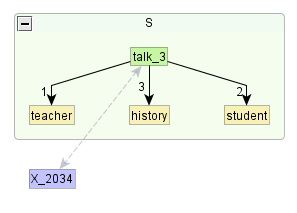
\includegraphics[width=0.4\textwidth, trim = {0cm 0.5cm 0cm 0cm},clip]{ch6/figs/root.png}
	\caption{Création de la racine à partir du n\oe{}ud dominant}
	\label{deroulement0}
\end{figure}


\subsection{Sélection du patron de régime dans le lexicon}
Ensuite, la règle \emph{actant\_gp\_selection} est déclenchée par l'apparition de \lex{talk\_3} pour satisfaire la racine. GenDR récupère les traits encodés pour chaque attribut \texttt{gp} de la classe verbale \texttt{talk-37.5}. Parmi ces \texttt{gp}, GenDR récupère ensuite le trait\texttt{id} dont la valeur est \texttt{NP\_V\_PP\_about\_topic\_PP\_to\_co\_agent} et le \texttt{dia} dont la valeur est \texttt{132}. Puis, il appose ces traits sur la racine.

\begin{figure}[htb]
	\centering
	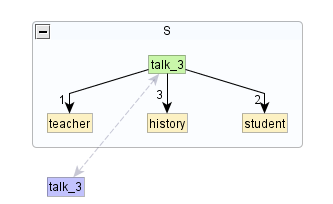
\includegraphics[width=0.4\textwidth, trim = {0.7cm 0.2cm 0cm 0cm},clip]{ch6/figs/selectiongp.png}
	\caption{Application de la règle actant\_gp\_selection}
	\label{deroulement1}
\end{figure}

\subsection{Application de la règle actancielle: \emph{actant\_gp\_ijk}}
La règle \emph{actant\_gp\_ijk} est sélectionnée puisque le trait de diathèse apposé sur le noeud précise qu'il y a trois actants sémantiques. À ce stade-ci, pour que l'arborisation se fasse correctement, il faut que les actants sémantiques imposés par la diathèse correspondent à ceux donnés par la structure sémantique. Comme notre exemple d'input en contient trois, alors la règle s'applique correctement et trois arcs en partance de la racine sont créés.

\begin{figure}[htb]
	\centering
	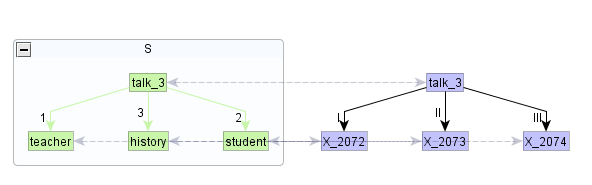
\includegraphics[width=1\textwidth, trim = {0cm 0.4cm 0cm 0cm},clip]{ch6/figs/actant_gp_ijk.png}
	\caption{Application d'une règle actancielle: actant\_gp\_ijk}
	\label{deroulement2}
\end{figure}

\subsection{Application des contraintes sur les n\oe{}uds}
La règle de contrainte récupère les restrictions sur les actants syntaxiques que sélectionne \texttt{talk-3-1.5} grâce au \texttt{id} d'un de ses \texttt{gp} qui renvoient aux propriétés du patron de régime dans le \emph{gpcon}: \lstinline|NP_V_PP_about_topic_PP_to_co_agent { I={rel=subjective dpos=N}, II=...| (voir \ref{gpexemple}). Dans ce cas, la règle d'application de contraintes s'applique trois fois puisqu'il y a trois n\oe{}uds vides.

\subsection{Lexicalisation des n\oe{}uds contraints}
On lexicalise tous les noeuds puisqu'ils en respectent les contraintes. Le système utilisera une règle de lexicalisation simple dans ce cas puisque chacun de ces sémantèmes existent dans le \emph{semanticon}.

\begin{figure}[htb]
	\centering
	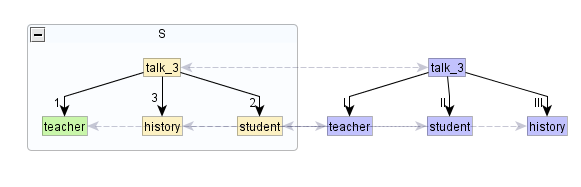
\includegraphics[width=1\textwidth, trim = {0cm 0.9cm 0cm 0cm},clip]{ch6/figs/lex.png}
	\caption{Applications d'une règle de lexicalisation: lex\_standard}
	\label{deroulement3}
\end{figure}

\subsection{Application de la règle \emph{actant\_gp\_selection}}
Finalement, la règle \emph{actant\_gp\_selection} est sollicitée pour les trois noeuds nouvellement lexicalisés \lex{teacher},\lex{student} et \lex{history}, bien que l'arbre profond semble complet à cette étape. Comme toutes les catégories syntaxiques du lexique ont des patrons de régime, le système récupère systématiquement les traits \texttt{id} et \texttt{dia} de chaque lexème dans l'arbre au cas où ceux-ci sélectionneraient des actants à leur tour. Ce qui n'est pas le cas dans cet exemple.

En ce qui concerne \textbf{l'arborisation de surface}, nous n'élaborerons pas sur cette partie puisqu'elle est quasi-identique à celle que nous avons vue dans la section \ref{sec:exemple} de GenDR. Les lexicalisations de surface sont effectuées par la même règle que nous avons expliquée, de même que la règle qui introduit les déterminants. Seules les règles actancielles de surface ont quelque peu changé, car elles puisent dorénavant l'information sur la correspondance entre les actants syntaxiques et les relations de surface qu'elles imposent (et le choix des prépositions) dans le \emph{gpcon}, alors que dans la version originale, le tout était encodé à même le \emph{lexicon}.

\begin{figure}[htb]
	\centering
	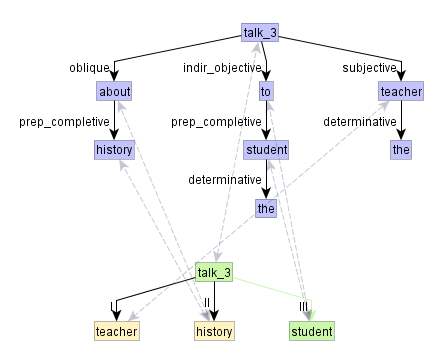
\includegraphics[width=0.6\textwidth, trim = {0cm 0cm 0cm 0cm},clip]{ch6/figs/ssynt.png}
	\caption{Applications des règles actancielles et réalisation des lexies fonctionnelles}
	\label{deroulement4}
\end{figure}

Cela met fin à notre chapitre sur l'adaptation de GenDR. Nous passerons maintenant à la phase d'évaluation.